% Capítulo 10: passadas da ordenação por seleção.
\documentclass[border=4pt]{standalone}
\usepackage[utf8]{inputenc}
\usepackage[T1]{fontenc}
% Estilo comum das figuras de vetores (capítulo 8).
\usepackage{tikz}
\usetikzlibrary{arrows.meta, positioning, calc, decorations.pathreplacing}
\definecolor{navy}{RGB}{23,45,80}
\definecolor{laranja}{RGB}{250,110,29}
\definecolor{cinzalogo}{RGB}{107,114,126}
\definecolor{azul}{RGB}{205,222,247}
\tikzset{
  casa/.style={draw=navy, line width=0.9pt, minimum width=8mm, minimum height=7mm,
               inner sep=0pt, font=\sffamily\small},
  pronta/.style={casa, fill=azul},
  parte/.style={casa, fill=laranja!12},
  marcada/.style={casa, fill=laranja!45, draw=laranja},
  fora/.style={casa, draw=cinzalogo!60, dashed, fill=white, text=cinzalogo!60},
  indice/.style={font=\sffamily\scriptsize, text=cinzalogo},
  explica/.style={font=\sffamily\small, text=navy, anchor=east},
  legenda/.style={font=\sffamily\scriptsize, text=cinzalogo},
  rotulo/.style={font=\sffamily\small\bfseries, text=navy},
  seta/.style={-{Stealth[length=2.2mm]}, navy, line width=0.9pt},
  chave/.style={decorate, decoration={brace, amplitude=4pt, mirror}, navy, line width=0.8pt},
}
% \vetor{nome}{x}{y}{valor/estilo, valor/estilo, ...}: casas lado a lado, chamadas nome0, nome1...
\newcommand{\vetor}[4]{%
  \foreach \valor/\estilo [count=\i from 0] in {#4} {
    \node[\estilo] (#1\i) at ($(#2, #3) + (\i*0.8, 0)$) {\valor};
  }
}

\tikzset{passo/.style={font=\sffamily\scriptsize, text=navy, anchor=west, align=left}}
\begin{document}
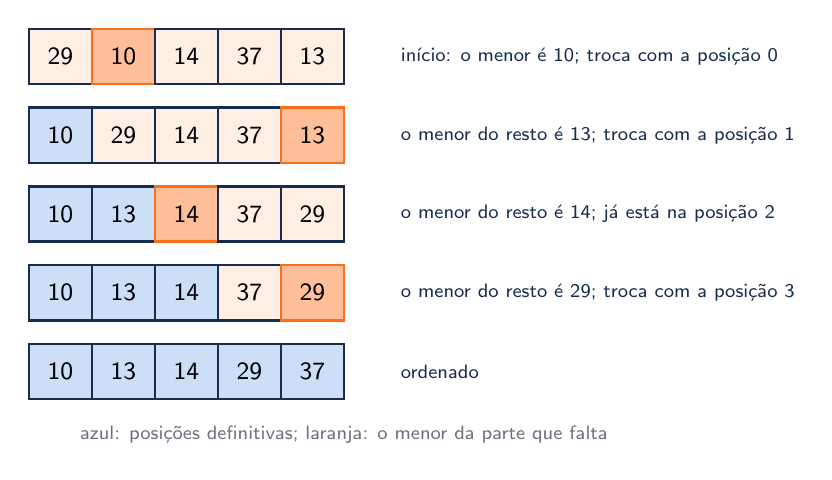
\begin{tikzpicture}
  \vetor{l0}{0}{0.0}{29/parte, 10/marcada, 14/parte, 37/parte, 13/parte}
  \node[passo] at (4.2, 0.0) {início: o menor é 10; troca com a posição 0};
  \vetor{l1}{0}{-1.0}{10/pronta, 29/parte, 14/parte, 37/parte, 13/marcada}
  \node[passo] at (4.2, -1.0) {o menor do resto é 13; troca com a posição 1};
  \vetor{l2}{0}{-2.0}{10/pronta, 13/pronta, 14/marcada, 37/parte, 29/parte}
  \node[passo] at (4.2, -2.0) {o menor do resto é 14; já está na posição 2};
  \vetor{l3}{0}{-3.0}{10/pronta, 13/pronta, 14/pronta, 37/parte, 29/marcada}
  \node[passo] at (4.2, -3.0) {o menor do resto é 29; troca com a posição 3};
  \vetor{l4}{0}{-4.0}{10/pronta, 13/pronta, 14/pronta, 29/pronta, 37/pronta}
  \node[passo] at (4.2, -4.0) {ordenado};
  \node[legenda] at (3.6, -4.8) {azul: posições definitivas; laranja: o menor da parte que falta};
\end{tikzpicture}
\end{document}
